\subsection{Body Separation of 10 mm}

The \(10~\mathrm{mm}\) separation case represents the weakest body-loading condition in this study. Although this distance is the largest spacing considered, it is still electrically small compared with the free-space wavelength at \(1.120~\mathrm{GHz}\). Therefore, measurable changes in impedance matching, efficiency, gain, and radiation pattern are still expected due to near-field coupling between the dipole and the lossy multilayer body model.

\subsubsection{Geometry and Simulation Setup}

The tuned free-space dipole length was kept fixed at

\[
L = 122.0~\mathrm{mm}.
\]

The wire radius was

\[
a = 0.905~\mathrm{mm},
\]

and the feed gap remained

\[
g = 2.0~\mathrm{mm}.
\]

For the \(10~\mathrm{mm}\) body-separation case, the air gap was defined as the distance between the lower surface of the cylindrical dipole wire and the top surface of the skin layer. Since the lower surface of the wire is located at

\[
z=-0.905~\mathrm{mm},
\]

the top of the skin layer was placed at

\[
z_{\mathrm{skin,top}}=-(10+0.905)
=
-10.905~\mathrm{mm}.
\]

The skin, fat, and muscle layers were then stacked downward in the negative \(z\)-direction. The tissue coordinates for this case were already summarized in Table~\ref{tab:body-10mm-coordinates}. The same material properties, layer thicknesses, boundary settings, and frequency range were used as described in the previous section.

The CST time-domain solver was used over the frequency range

\[
0.7~\mathrm{GHz} \leq f \leq 1.5~\mathrm{GHz}.
\]

A far-field monitor was defined at the target frequency,

\[
f_0 = 1.120~\mathrm{GHz}.
\]

The extracted results include the return loss \(S_{11}\), radiation efficiency, total efficiency, gain, and two-dimensional and three-dimensional radiation patterns.

The CST geometry for the \(10~\mathrm{mm}\) separation case is shown in Figure~\ref{fig:body-10mm-geometry}.

\begin{figure}[H]
\centering
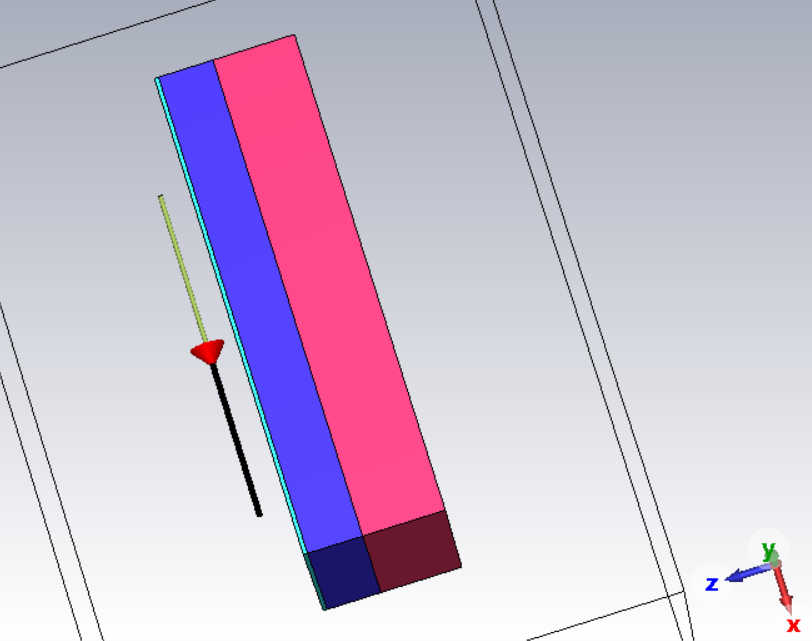
\includegraphics[width=0.82\textwidth]{figures/body_10mm/geometry_body_10mm_side_view.png}
\caption{CST side-view geometry for the \(10~\mathrm{mm}\) antenna-body separation case.}
\label{fig:body-10mm-geometry}
\end{figure}

\subsubsection{Return-Loss Result}

The CST return-loss result for the \(10~\mathrm{mm}\) body-separation case showed that the dominant matching minimum shifted below the target frequency. The minimum \(S_{11}\) occurred at

\[
f_{\min} = 1.0312~\mathrm{GHz},
\]

with

\[
S_{11,\min} = -10.49934~\mathrm{dB}.
\]

At the target frequency of \(1.120~\mathrm{GHz}\), the return loss was

\[
S_{11}(1.120~\mathrm{GHz}) = -7.839072~\mathrm{dB}.
\]

\begin{table}[htbp]
\centering
\caption{Return-loss result for the \(10~\mathrm{mm}\) body-separation case.}
\label{tab:body-10mm-s11-result}
\begin{tabular}{lc}
\hline
\textbf{Quantity} & \textbf{Value} \\
\hline
Dipole length & \(122.0~\mathrm{mm}\) \\
Antenna-body separation & \(10~\mathrm{mm}\) \\
Minimum-\(S_{11}\) frequency & \(1.0312~\mathrm{GHz}\) \\
Minimum \(S_{11}\) & \(-10.49934~\mathrm{dB}\) \\
\(S_{11}\) at \(1.120~\mathrm{GHz}\) & \(-7.839072~\mathrm{dB}\) \\
\hline
\end{tabular}
\end{table}

Compared with the tuned free-space case, the antenna no longer satisfies the \(-10~\mathrm{dB}\) matching criterion at the target frequency. The tuned free-space dipole had

\[
S_{11}(1.120~\mathrm{GHz}) = -15.48433~\mathrm{dB},
\]

whereas the \(10~\mathrm{mm}\) body case produced

\[
S_{11}(1.120~\mathrm{GHz}) = -7.839072~\mathrm{dB}.
\]

This degradation indicates that the lossy body model perturbs the antenna input impedance even at the largest separation distance considered in this project.

The return-loss response for the \(10~\mathrm{mm}\) body-loading case is shown in Figure~\ref{fig:body-10mm-s11}.

\begin{figure}[htbp]
\centering
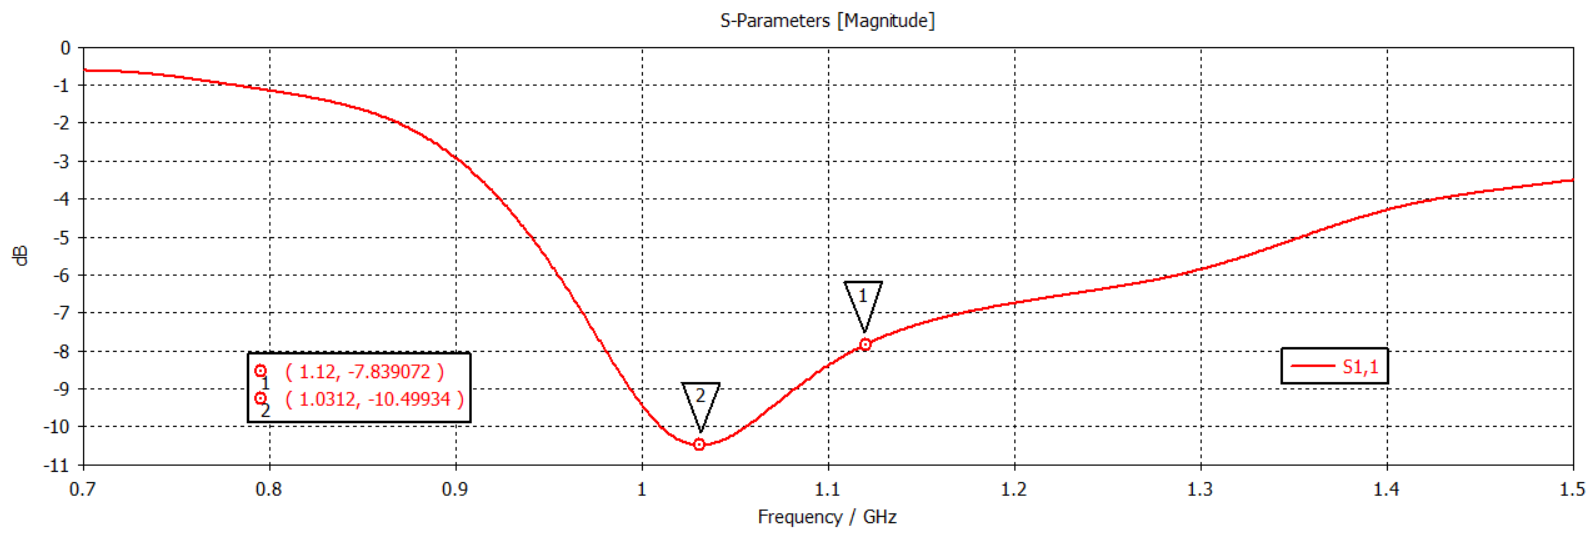
\includegraphics[width=0.82\textwidth]{figures/body_10mm/s11_body_10mm_with_markers.png}
\caption{Return loss for the \(10~\mathrm{mm}\) body-separation case. The dominant matching minimum occurs at \(1.0312~\mathrm{GHz}\), while \(S_{11}\) at \(1.120~\mathrm{GHz}\) is \(-7.839072~\mathrm{dB}\).}
\label{fig:body-10mm-s11}
\end{figure}

\subsubsection{Efficiency and Gain Result}

The far-field result at \(1.120~\mathrm{GHz}\) showed that the nearby body reduced the radiating performance of the antenna. CST reported the following values:

\[
\eta_{\mathrm{rad}} = -3.410~\mathrm{dB},
\]

\[
\eta_{\mathrm{tot}} = -4.190~\mathrm{dB},
\]

and

\[
G = 0.7515~\mathrm{dBi}.
\]

\begin{table}[htbp]
\centering
\caption{Efficiency and gain result for the \(10~\mathrm{mm}\) body-separation case at \(1.120~\mathrm{GHz}\).}
\label{tab:body-10mm-efficiency-gain}
\begin{tabular}{lc}
\hline
\textbf{Quantity} & \textbf{Value} \\
\hline
Radiation efficiency & \(-3.410~\mathrm{dB}\) \\
Total efficiency & \(-4.190~\mathrm{dB}\) \\
Gain & \(0.7515~\mathrm{dBi}\) \\
\hline
\end{tabular}
\end{table}

The radiation efficiency reduction is caused by power absorption in the lossy tissue layers. The total efficiency is lower than the radiation efficiency because it also includes impedance mismatch at the target frequency. Therefore, both tissue loss and mismatch contribute to the reduced antenna performance.

\begin{figure}[htbp]
\centering
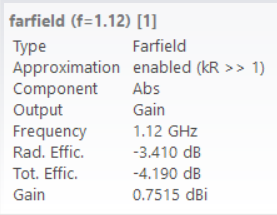
\includegraphics[width=0.42\textwidth]{figures/body_10mm/farfield_parameters_body_10mm.png}
\caption{CST far-field parameter summary for the \(10~\mathrm{mm}\) body-separation case at \(1.120~\mathrm{GHz}\).}
\label{fig:body-10mm-farfield-parameters}
\end{figure}

\subsubsection{Radiation Pattern Observation}

The far-field monitor at \(1.120~\mathrm{GHz}\) was used to evaluate the radiation behavior of the complete antenna-body system. Although the body is located in the near-field region of the dipole, the CST far-field result represents the far-zone radiation pattern after the near-field interaction between the antenna and the body has been solved.

For the \(10~\mathrm{mm}\) case, the radiation pattern remained broadly dipole-like, but the presence of the lossy body model modified the field distribution and reduced the maximum gain. The body acts both as a high-permittivity loading structure and as a lossy absorber. As a result, part of the accepted power is dissipated in the tissue layers instead of being radiated into the far field.

The three-dimensional gain pattern at \(1.120~\mathrm{GHz}\) is shown in Figure~\ref{fig:body-10mm-3d-pattern}.

\begin{figure}[htbp]
\centering
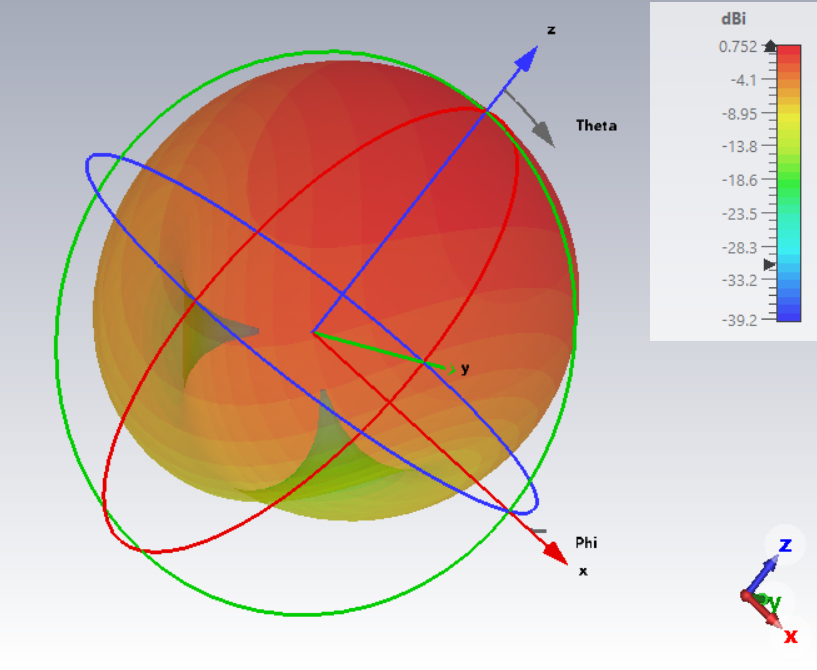
\includegraphics[width=0.82\textwidth]{figures/body_10mm/pattern_3d_gain_body_10mm.png}
\caption{Three-dimensional gain pattern for the \(10~\mathrm{mm}\) body-separation case at \(1.120~\mathrm{GHz}\).}
\label{fig:body-10mm-3d-pattern}
\end{figure}

The E-plane and H-plane radiation-pattern cuts for the \(10~\mathrm{mm}\) body-separation case are shown in Figures~\ref{fig:body-10mm-2d-phi0} and~\ref{fig:body-10mm-2d-phi90}, respectively. Since the dipole is oriented along the \(x\)-axis, the \(\phi=0^\circ\) cut corresponds to the \(x\)-\(z\) principal plane, or E-plane, while the \(\phi=90^\circ\) cut corresponds to the \(y\)-\(z\) principal plane, or H-plane.

\begin{figure}[htbp]
\centering
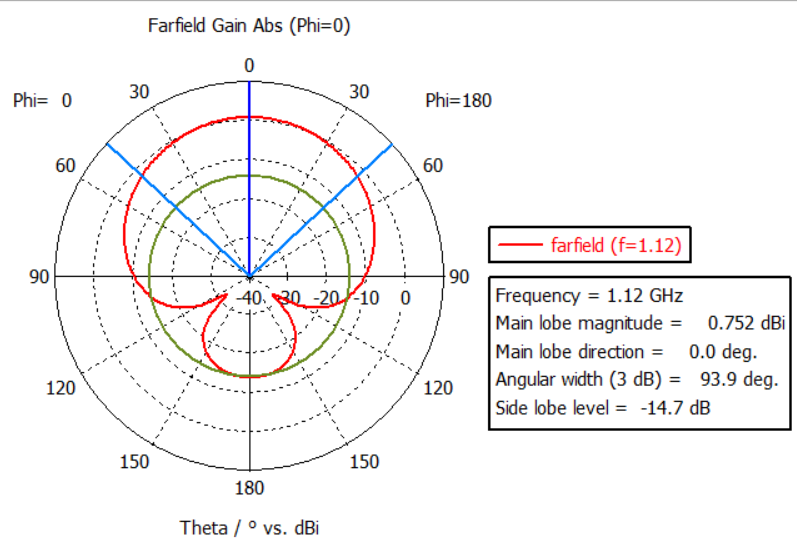
\includegraphics[width=0.82\textwidth]{figures/body_10mm/pattern_2d_body_10mm_phi0.png}
\caption{E-plane radiation-pattern cut for the \(10~\mathrm{mm}\) body-separation case at \(1.120~\mathrm{GHz}\). This cut corresponds to \(\phi=0^\circ\), or the \(x\)-\(z\) principal plane.}
\label{fig:body-10mm-2d-phi0}
\end{figure}

\begin{figure}[htbp]
\centering
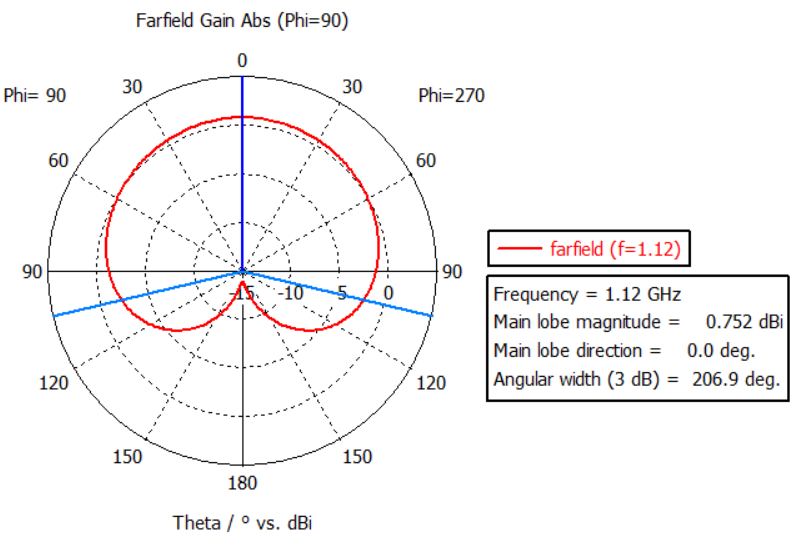
\includegraphics[width=0.82\textwidth]{figures/body_10mm/pattern_2d_body_10mm_phi90.png}
\caption{H-plane radiation-pattern cut for the \(10~\mathrm{mm}\) body-separation case at \(1.120~\mathrm{GHz}\). This cut corresponds to \(\phi=90^\circ\), or the \(y\)-\(z\) principal plane.}
\label{fig:body-10mm-2d-phi90}
\end{figure}

\subsubsection{Interpretation of the 10 mm Case}

The \(10~\mathrm{mm}\) body-separation case shows the first clear evidence of body loading. Relative to the tuned free-space antenna, the matching minimum shifted from approximately

\[
1.1168~\mathrm{GHz}
\]

to

\[
1.0312~\mathrm{GHz}.
\]

This downward shift indicates that the nearby high-permittivity tissue layers increased the effective electrical loading of the dipole. In other words, the antenna behaves electrically longer when placed near the body.

At the target frequency, the return loss degraded from

\[
-15.48433~\mathrm{dB}
\]

in free space to

\[
-7.839072~\mathrm{dB}
\]

with the body at \(10~\mathrm{mm}\). The gain was also reduced to

\[
0.7515~\mathrm{dBi}.
\]

These results confirm that even a \(10~\mathrm{mm}\) separation is close enough for the body to significantly affect the input matching and radiating performance of the wearable dipole antenna.
